\section{Large Language Models}
\glspl{llm} are advanced systems capable of understanding and producing human language. They are designed to process text in a way that captures meaning and context, allowing them to generate coherent and relevant responses or content. Essentially, LLMs can “read” and “write” in a manner that closely resembles human communication. The utility of LLMs lies in their versatility. They can assist in generating written content, providing summaries, or creating explanations on complex topics. They are also used in conversational contexts, offering guidance, answering questions, or engaging in dialogue with users. Beyond communication, LLMs support decision-making and information management by extracting insights from large amounts of text or presenting information in an easily understandable form. In essence, LLMs act as intelligent language assistants, capable of understanding human expression and aiding in tasks that involve reading, writing, or reasoning with text, making them valuable across many areas of work and daily life.

\subsection{Evolution of Large Language Models.} 
The evolution of Language Models into modern \glspl{llm} traces a path from early statistical estimation to advanced neural architectures and alignment techniques \cite{wang2024historydevelopmentprincipleslarge}. Initially, Language Models were understood as probabilistic models of natural language, estimating the likelihood of word sequences, with early n-gram models relying on the Markov assumption to approximate the probability of the next word based on a small preceding context, but suffering from data sparsity and a lack of semantic understanding. 

The introduction of neural networks reframed next-word prediction as a classification problem, augmented by word embeddings that captured semantic relationships in dense vector spaces, replacing sparse one-hot encodings, and enabling recurrent architectures such as RNNs and LSTMs \cite{SHERSTINSKY2020132306} to handle longer contexts. 

A transformative advance occurred with the Transformer architecture \cite{transformers}, which addressed long-term dependency limitations and allowed parallelizable processing through the self-attention mechanism, giving rise to decoder-only Transformers exemplified by the GPT family. Models like GPT-2 \cite{radford2019gpt2} and GPT-3 \cite{brown2020gpt3} dramatically scaled parameters (GPT-3 reaching 175B) and training data, confirming scaling laws and demonstrating few-shot in-context learning, while highlighting inefficiencies in oversized yet undertrained models. 

This prompted compute-optimal training, as in Chinchilla \cite{hoffmann2022chinchilla} (70B parameters), which achieved superior performance by training on more tokens rather than simply increasing model size. 

The final evolutionary step involved aligning LLMs with human preferences and practical utility, formalized through instruction tuning (improving zero-shot generalization, demonstrated by FLAN \cite{chung2022flan} and Reinforcement Learning with Human Feedback (RLHF) as implemented in InstructGPT \cite{openai2022instructgpt}, producing models that are Helpful, Honest, and Harmless (HHH). 

This trajectory characterizes current accessible LLMs, including the LLaMA family \cite{touvron2023llama}, which combine massive scale, semantic understanding, and alignment strategies to serve as powerful, instruction-tuned conversational agents.
The Figure \ref{fig:llmevo} gives an idea of the exponential growth of the llm models in the last years.

\begin{figure}[ht]
    \centering
    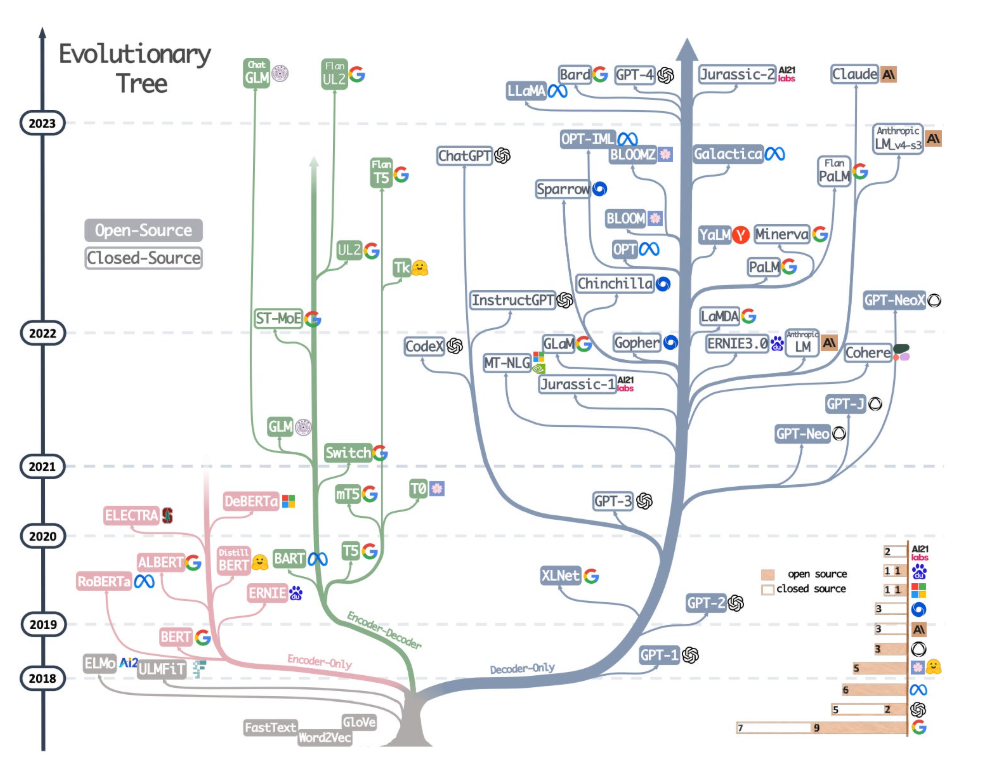
\includegraphics[width=1\textwidth]{chap2/figure/llm_evo.png}
    \caption{The evolution of LLMs \cite{interconnects_llm_evolution}.}
    \label{fig:llmevo}
\end{figure}



\subsection{The Attention mechanism}

The attention mechanism, which is central to LLMs, allows the model to dynamically assign relevance to different tokens within an input sequence. This mechanism overcomes the limitations of sequential architectures by enabling long-range dependencies to be captured efficiently. Specifically, self-attention computes pairwise interactions between all tokens in the sequence, permitting each token to attend to any other regardless of positional distance. The Figure \ref{fig:atte} shows a visual example of attention computed in the context of words translation.  

The core computation is the scaled dot-product attention. Given input token embeddings, three matrices are derived through parameterized linear projections: queries \( Q \), keys \( K \), and values \( V \). The attention output is formulated as:
\[
\text{Attention}(Q,K,V) = \text{softmax}\left(\frac{Q K^\top}{\sqrt{d_k}}\right) V
\]
where \( d_k \) is the dimensionality of the key vectors and serves as a scaling factor to stabilize gradients during training. The softmax normalizes the similarity scores into a probability distribution, highlighting the most relevant tokens for each query.

Multi-head attention extends this formulation by computing several parallel attention outputs, each with its own learned projections. These outputs are concatenated and linearly transformed to produce the final attended representation, enabling the model to capture different semantic and syntactic aspects concurrently.

This architecture forms the basis of Transformers that power state-of-the-art LLMs like GPT-4 of OpenAI and Cloude 4.5 of Anthropic\cite{transformers,soydaner2022attention}.

\begin{figure}[ht]
    \centering
    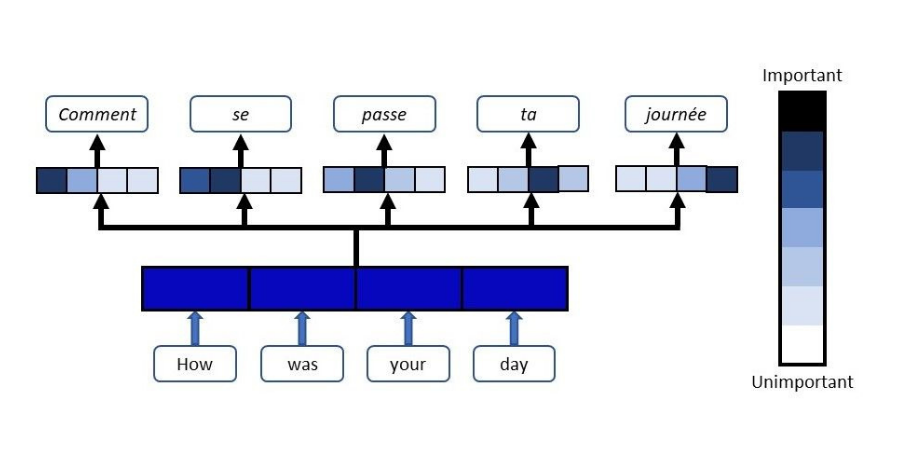
\includegraphics[width=1\textwidth]{chap2/figure/attention.png}
    \caption{A high level representation of the attention \cite{medium_attention_mechanism}.}
    \label{fig:atte}
\end{figure}



\subsection{Applications of LLMs.}
LLMs have become increasingly prominent across research and industry, owing to their ability to generate, analyze, and adapt human-like text for a wide variety of purposes \cite{naveed2024comprehensiveoverviewlargelanguage}. Their versatility extends from routine tasks, such as drafting emails, translating text, or summarizing documents, to more advanced applications involving programming assistance, data analysis, and content generation. This adaptability makes LLMs not only useful as personal assistants or customer service agents but also as tools capable of managing and interpreting vast amounts of information that would otherwise demand significant human effort.

In medicine, for instance, LLMs are beginning to reshape both healthcare delivery and research practices. By analyzing patient records alongside extensive medical literature, they can provide clinicians with evidence-based recommendations, support diagnostic reasoning, and suggest treatment strategies. Beyond clinical practice, they facilitate patient engagement through conversational interfaces, offer scalable tools for medical education such as training simulations and tailored learning resources, and contribute to public health initiatives by detecting outbreaks, monitoring social responses, and disseminating accurate health information \cite{naveed2024comprehensiveoverviewlargelanguage}.

A similar transformative role is emerging in education. LLMs enable personalized learning by adapting materials to individual needs, while simultaneously assisting teachers with tasks such as lesson planning, grading, and developing accessible content. They are particularly effective in language learning, where they act as interactive conversation partners, capable of correcting grammar, guiding vocabulary use, and enhancing fluency. By providing transcription services for the hearing impaired or simplifying complex texts for learners with difficulties, they also make education more inclusive.

In the sciences, LLMs help researchers navigate overwhelming volumes of literature by summarizing findings, highlighting patterns, and even generating new hypotheses. Their ability to assist in drafting manuscripts and standardizing formatting further supports the research process, allowing teams across disciplines to communicate more effectively. In mathematics, they complement this role by breaking down complex problems, offering step-by-step explanations, and aiding in the verification of proofs, thus bridging the gap between abstract theory and applied contexts.

The legal field also benefits from LLMs, particularly in the processing and interpretation of extensive documentation. They can analyze case law, explain legal terminology, and support reasoning tasks, with domain-specific fine-tuning significantly enhancing their accuracy and practical utility. A similar pattern is seen in finance, where models, such as FinGPT\cite{yang2023fingptopensourcefinanciallarge}, demonstrate the value of tailoring LLMs to industry-specific data. These systems support applications ranging from robo-advising and algorithmic trading to more complex decision-making, highlighting the importance of customization for high-stakes domains.

Finally, robotics represents another promising area of integration. Here, LLMs improve human-robot interaction by enabling robots to understand instructions in natural language and plan tasks accordingly. Their capacity to integrate information from diverse sources also equips robots with the ability to adapt to new environments, acquire new skills, and operate more collaboratively alongside humans \cite{naveed2024comprehensiveoverviewlargelanguage}.

Taken together, these applications illustrate how LLMs extend human capabilities and introduce efficiencies across domains as diverse as healthcare, education, law, science, and robotics. Yet, their rapid adoption also raises important challenges concerning data quality, bias, and explainability. Addressing these issues will be essential if LLMs are to realize their full potential as reliable and responsible tools for advancing research, industry, and society.




\subsection{Training Paradigms.}
LLMs are developed through a multi-stage training process that enables them to acquire linguistic knowledge and adapt to different tasks. This process generally includes three main phases: \textit{pretraining}, \textit{fine-tuning}, and \textit{instruction tuning}.  

In the first phase, known as \textit{pretraining}, the model is exposed to very large collections of unlabelled text data, as explained by \cite{johnson2024primerlargelanguagemodels}. During this stage, the model learns through self-supervised objectives that do not require human annotation. Two common objectives are causal language modeling \cite{micheletti2024explorationmaskedcausallanguage}, which trains the model to predict the next token in a sequence as seen in GPT models, and masked language modeling\cite{micheletti2024explorationmaskedcausallanguage}, which teaches the model to reconstruct hidden tokens within a sentence as used in BERT. Through this large-scale learning process, the model develops an extensive understanding of grammar, meaning, context, and factual knowledge.  

After pretraining, the model is adapted through \textit{fine-tuning}. In this phase, the model is trained on smaller, labeled datasets that focus on specific domains or applications \cite{pretraining}. Fine-tuning allows the model to apply its general linguistic and semantic knowledge to specialized tasks such as legal text analysis, biomedical literature summarization, or program code generation. This step improves accuracy and relevance within the target domain.  

The third phase, \textit{instruction tuning}, aims to make LLMs more responsive to human instructions written in natural language\cite{instructiontuning}. Instead of using datasets designed for a single task, instruction tuning relies on large collections of examples where each task is paired with a clear written instruction, such as “Translate this subsection into French” or “Summarize this article in three sentences.” These instructions are called \textit{prompts}. A prompt is an input text provided to the model that specifies the task or desired output. It serves as a guide that tells the model what to do and how to respond in context.  

By learning from many such examples, instruction-tuned models acquire the ability to generalize to new tasks that they have never encountered before. This ability, known as \textit{zero-shot generalization}, allows users to interact with models simply by providing well-formulated prompts. As a result, instruction tuning has become a key step in developing LLMs that are more practical, interactive, and adaptable to real-world applications.



\subsection{State-of-the-Art Large Language Models.}  
The development of LLMs by leading organizations has profoundly influenced both research and practical applications in artificial intelligence. Companies such as OpenAI, Anthropic, Google, and Mistral have introduced models that differ in scale, architecture, and focus, collectively shaping the state of the art. OpenAI's GPT series, for instance, has emphasized versatility and multimodal capabilities. Anthropic's Claude models prioritize safety and alignment, reflecting growing concerns about ethical AI and reliable instruction-following. Google’s PaLM series has focused on scale and multilingual performance, demonstrating how massive models trained on extensive datasets can achieve competitive reasoning and language understanding across diverse tasks. Open-source initiatives such as Mistral complement these proprietary developments by providing accessible models with optimized architectures, encouraging experimentation, transparency, and reproducibility in research.

Across these platforms, the benefits of modern LLMs are evident. They provide high-quality natural language understanding, reasoning, and generation, and support a wide range of tasks, from summarization and translation to coding assistance and domain-specific problem solving. Their availability, whether as API-accessible proprietary systems or fully open-source models, facilitates rapid prototyping and deployment in both academic and industrial contexts. At the same time, limitations remain. Even state-of-the-art models can produce hallucinations, display biases inherited from training data, and underperform on tasks requiring nuanced domain knowledge or low-resource language proficiency. Moreover, proprietary models often impose access and cost constraints, while open-source models shift the burden of deployment, fine-tuning, and computational resources onto the user. 

In sum, the current landscape reflects a dynamic interplay between capability, accessibility, and responsibility. The evolution of LLMs illustrates both the technical progress achieved by leading companies and the ongoing challenges in reliability, fairness, and ethical deployment. Understanding these trends is crucial for positioning research and applications within a rapidly developing and heterogeneous AI ecosystem \cite{gpt4_technical_report, anthropic_claude_4, palm_2022, mistral_7b}.







\subsection{Limitations of LLMs.}
Despite their impressive capabilities, Large Language Models have several inherent limitations \cite{limitationsLLM}. First, they can generate information that appears confident but is factually incorrect, which poses challenges in reliability and trust. Second, they are prone to biases, reflecting patterns present in their training data, which can result in unfair, offensive, or otherwise undesirable outputs. Third, LLMs do not truly understand the content they produce; they rely on patterns in language rather than reasoning or comprehension, limiting their ability to perform complex logical or causal inference. Additionally, their responses can sometimes be inconsistent or sensitive to small changes in input phrasing. Finally, LLMs require significant computational resources for training and deployment, which can limit accessibility and environmental sustainability. Recognizing these limitations is crucial when applying LLMs in real-world contexts, and it highlights the need for careful supervision, evaluation, and ethical consideration.

